
\documentclass{article}
\usepackage{hyperref}

\usepackage{graphicx}

\title{Fiberassign performance}
\author{Jaime E. Forero-Romero \footnote{{\texttt{j.e.forero.romero@gmail.com}}}\\Universidad de los Andes}
\date{\today}

\begin{document}
\maketitle
\begin{abstract}
In this document I use DR7 data to calculate the conditions under
which fiberassign meets the desired performance in terms of total
fiber usage and number of calibration targets. 
The places where these metrics are not met is due to the low number of
calibration targets (sky or standard stars).  
Taking into account the current variability of number densities for
calibration and science targets across DR7 only $47\%$ of the 7054
tiles meet all the requirements. 
The recomendation is to increase the number of standards above 290
locations per tile and good sky locations above 18500 per tile.
\end{abstract}

\section{Introduction}
{\texttt fiberassign} is the software that computes the assignment of
fibers to DESI targets. 

The following are the minimal requirements on its performance
\begin{itemize}
\item Fiber assignment uses required fraction of fibers IN.DAT-7002
\item Fiber assignment provides sufficient calibration fibers IN.DAT-7003
\end{itemize}

In this document I present the results of running {\texttt
  fiberassign} on targets from DR7 to demonstrate how the two
requirements mentioned above are met. 
Furthermore I list some computational performance results to
understand how long does it take to run the code and how many
resources does it use.

\section{Software and input data}

For this report I use tag {\texttt 0.10.1} of {\texttt fiberassign}. 

The input targetting data comes from DR7. On NERSC the files can be found here:
{\texttt{/project/projectdirs/desi/target/catalogs/dr7.1/PR372/}}

The targeting files need to be prepared in order to pass them to
fiberassign.
The code that prepares the data and runs fiberassign can be found
here:
\url{https://github.com/forero/fiberassign_explore/blob/master/py/fiberassign_on_DR7.py}.
The script needs to be executed as {\texttt{python fiberassign\_on\_DR7.py --program dark
--size large}} to produce the outputs analized in this report.

The most important features to highlight about fiberassign are the
following:

\begin{itemize}
\item It receives as input three files: a list of science targets, a
  list of good sky locations and a list of standard
  stars. 
\item The code fills up to 400 sky fibers and 100 std fibers if the
  number density of those calibration targets is high enough.
\item Afterwards the code proceeds to assign science targets.
\item If there are unused fibers after the science assignment process
  those fibers are filled with sky targets if available.
\item There are also BADSKY locations that are treated as another
  science target with the lowest priority.
\end{itemize}

\section{Results}


We only use targets that can be observed in dark time. 
With this restriction we end up with 7054 DESI tiles that correspond
to dark time and overlap with the DR7.1 footprint. 
This selection returns 36M targets, 1.3M standard stars and
22M sky locations.

Upper panel in Figure \ref{fig:used_fibers} shows the location of all
tiles that use all fibers, lower panel shows the tiles that use less
than 5000 fibers.
Only 3374 tiles (less than half) use all its fibers, the remaining
3680 tiles use varying number of fibers: from a few hundreds to 4999. 

The regions at high declination use a low fraction of fibers due to a
low number of targets. 
This case is ilustrated in Figure
\ref{fig:tile_low_fraction}. 
However, there is a large fraction of tiles with numbers of $\approx
4990$ fibers used.
Figure \ref{fig:tile_high_fraction} illustrates this case  where most
of the fibers go to clustered BADSKY locations, this indicates that
there are not enough SKY and science targets to fill up the fibers.



Figures \ref{fig:used_sky_fibers} and \ref{fig:used_std_fibers} show
the regions with usages above and below the expected values for SKY
and STD fibers.
For SKY 6208 tiles meet the requirements, while for STD 5896 tiles
meet the requirements. 
The number of tiles meeting both requirements is 5853, that is $82\%$ of
the tiles.
The number of tiles meeting the SKY+STD requirements and using all the
fibers is 3359, that is $47\%$ of the tiles.

Figures \ref{fig:std_dens} and \ref{fig:sky_dens} show the number of
STD/SKY fibers in a tile as a function of the STD/SKY density,
respectively.
These Figures show that the minimal number of STD targets required not
to miss the performance goal is 290 standards per tile, while for SKY locations the
minimum is 9300 per tile. 

We also find that in locations with science densities above 30000
targets per tile and 290 STD targets per tile, the sky locations must
be higher than 18500 to achieve full usage of all fibers.



\begin{figure}[!h]
\begin{center}
\begin{center}
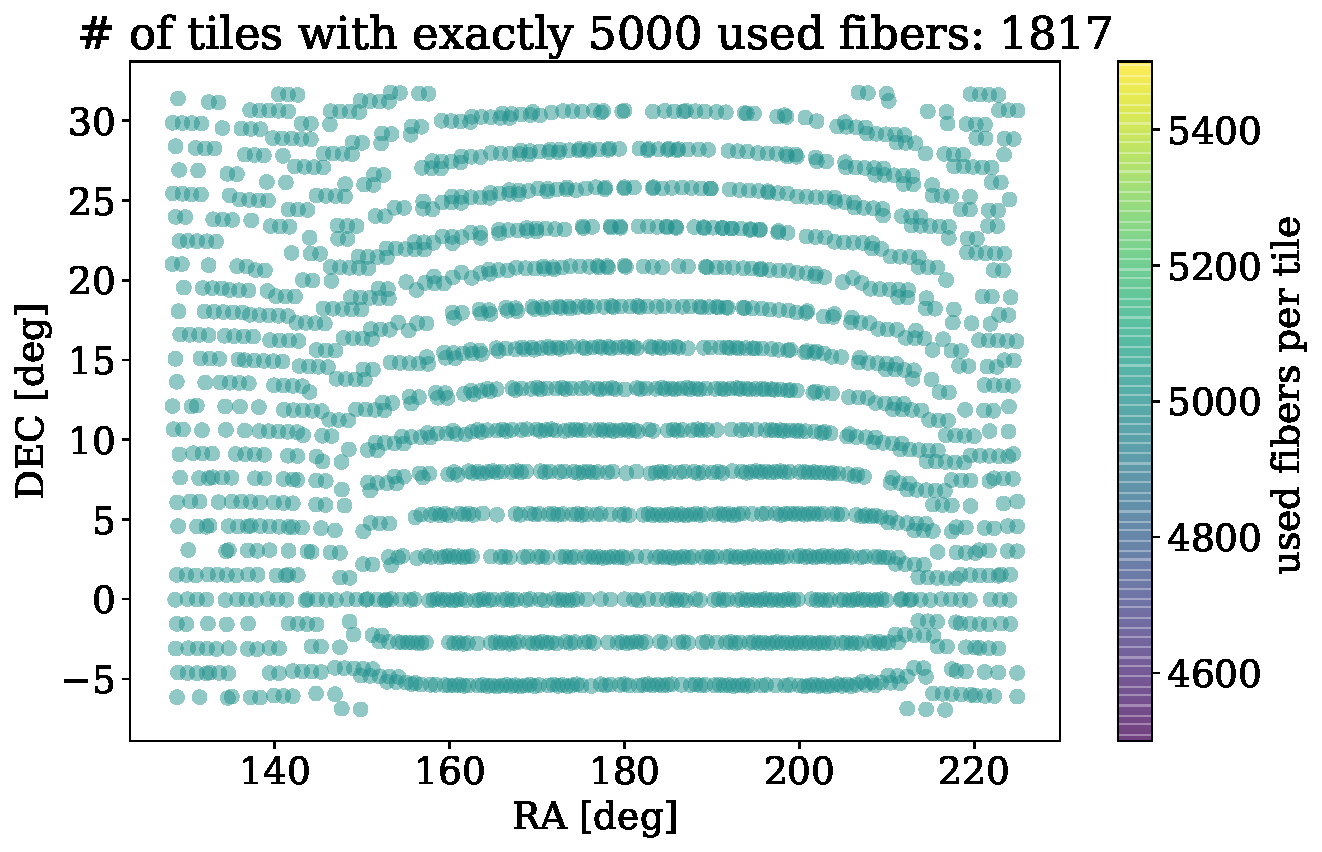
\includegraphics[scale=0.50]{assigned_used_ra_dec_exact.pdf}
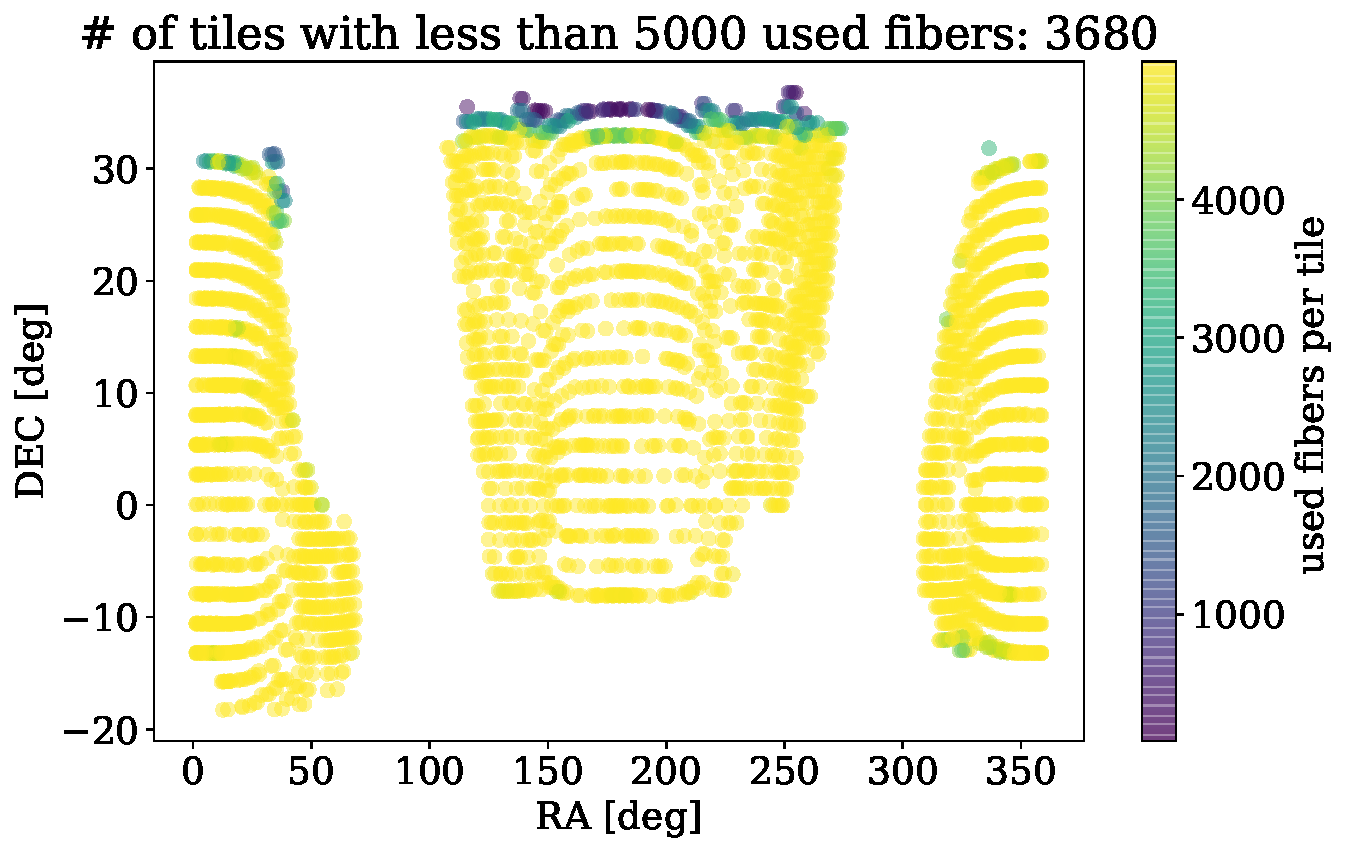
\includegraphics[scale=0.50]{assigned_used_ra_dec_below.pdf}
\end{center}
\caption{ Upper panel: location of the tiles that allocate all 5000
  fibers. 
Lower panel: location of the tiles that use less than 5000 fibers.
\label{fig:used_fibers}}
\end{center}
\end{figure}


\begin{figure}[!h]
\begin{center}
\begin{center}
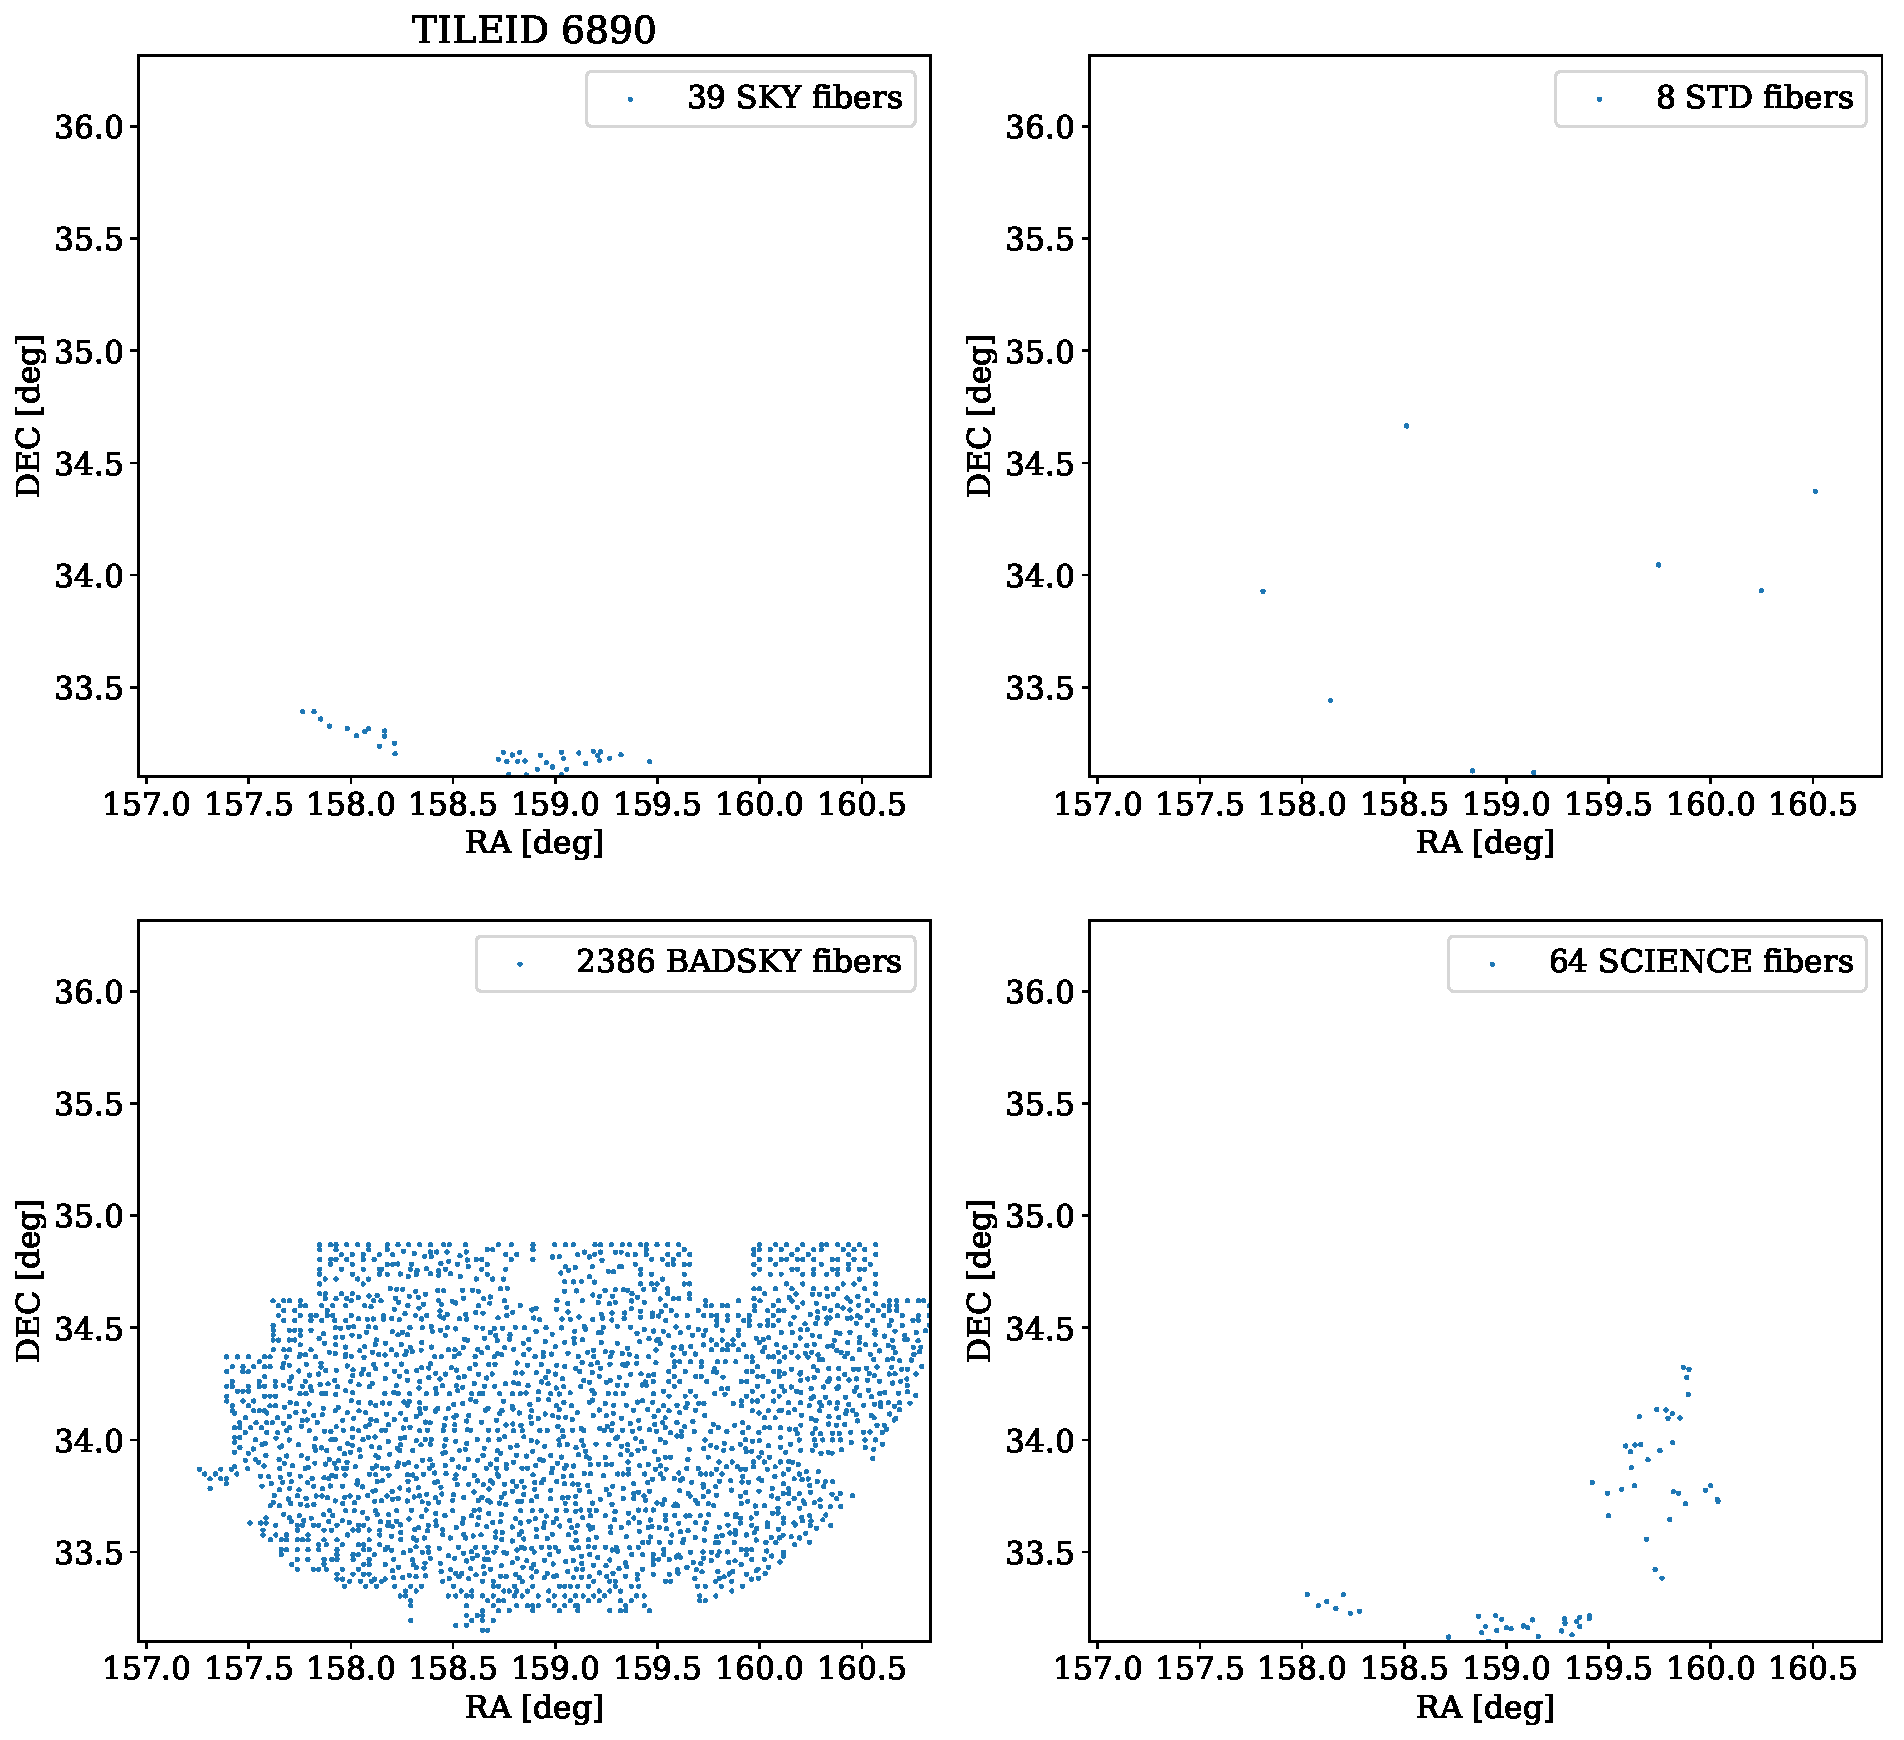
\includegraphics[scale=0.40]{single_tile_6890.pdf}
\end{center}
\caption{Tile with a low fraction ($50\%$) of used fibers.
Each panel shows the different kinds of targets that are
assigned. There is a clear lack of targets above 35 degrees of
declination. 
\label{fig:tile_low_fraction}}
\end{center}
\end{figure}

\begin{figure}[!h]
\begin{center}
\begin{center}
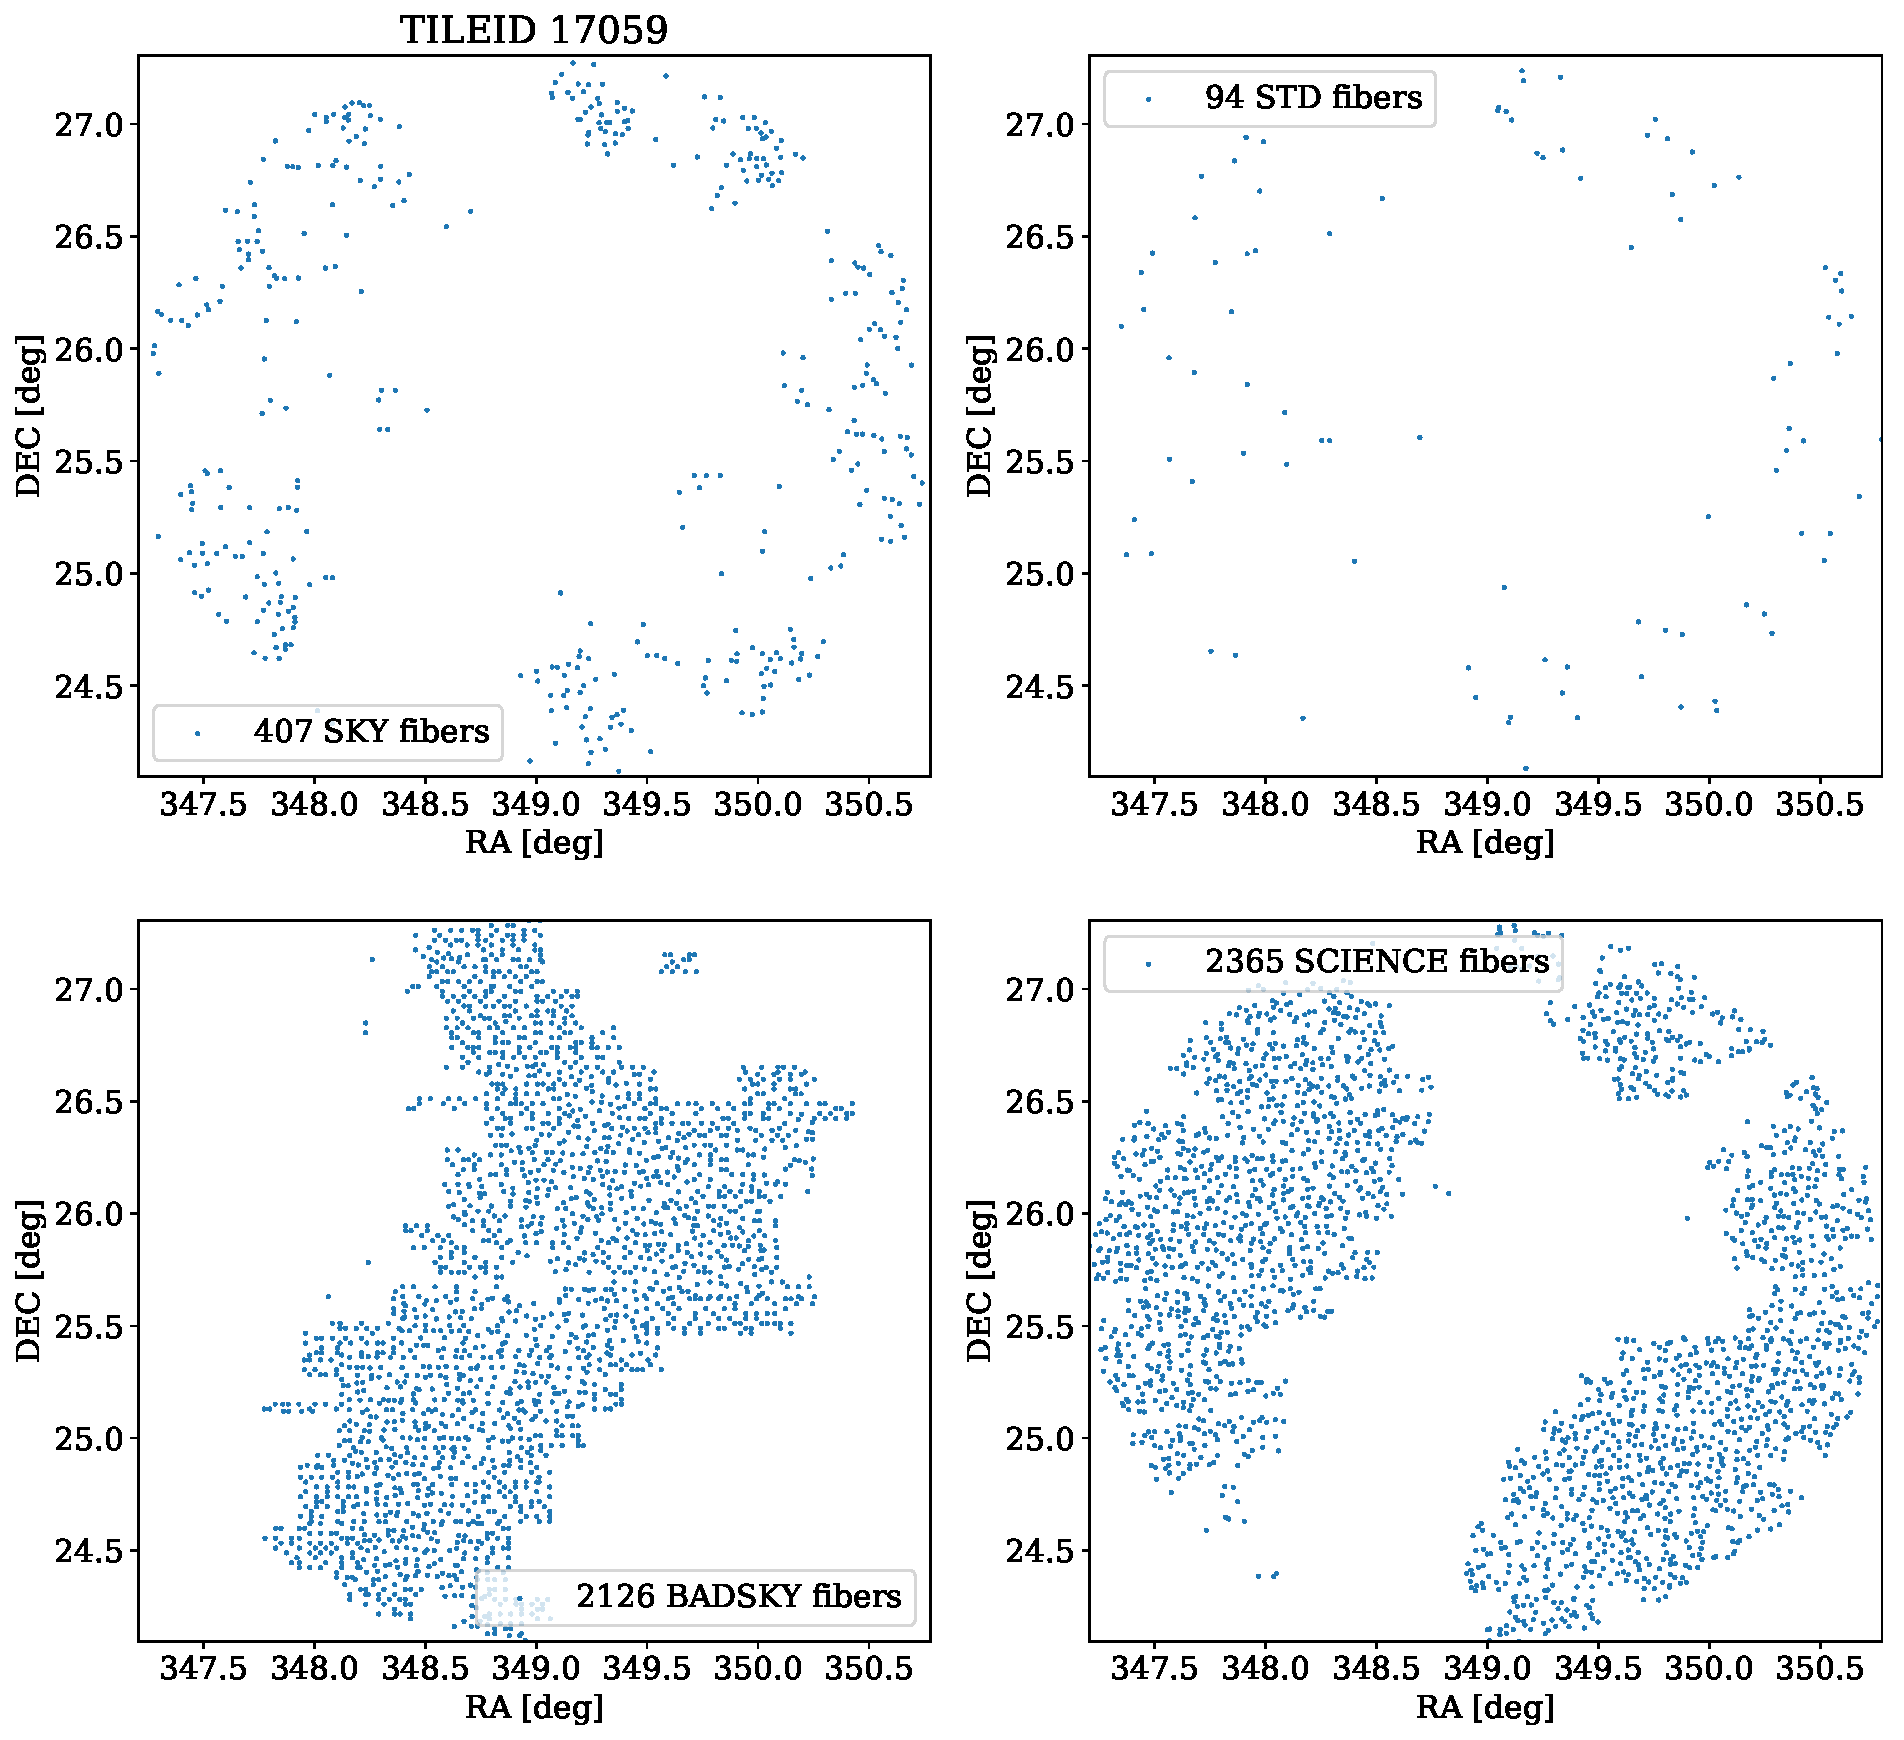
\includegraphics[scale=0.40]{single_tile_17059.pdf}
\end{center}
\caption{Tile with a high fraction ($99\%$ but not $100\%$) of used fibers.
Each panel shows the different kinds of targets that are
assigned. 
Mostly BADSKY location seems to be available in this region of the
sky. 
\label{fig:tile_high_fraction}}
\end{center}
\end{figure}


\begin{figure}[!h]
\begin{center}
\begin{center}
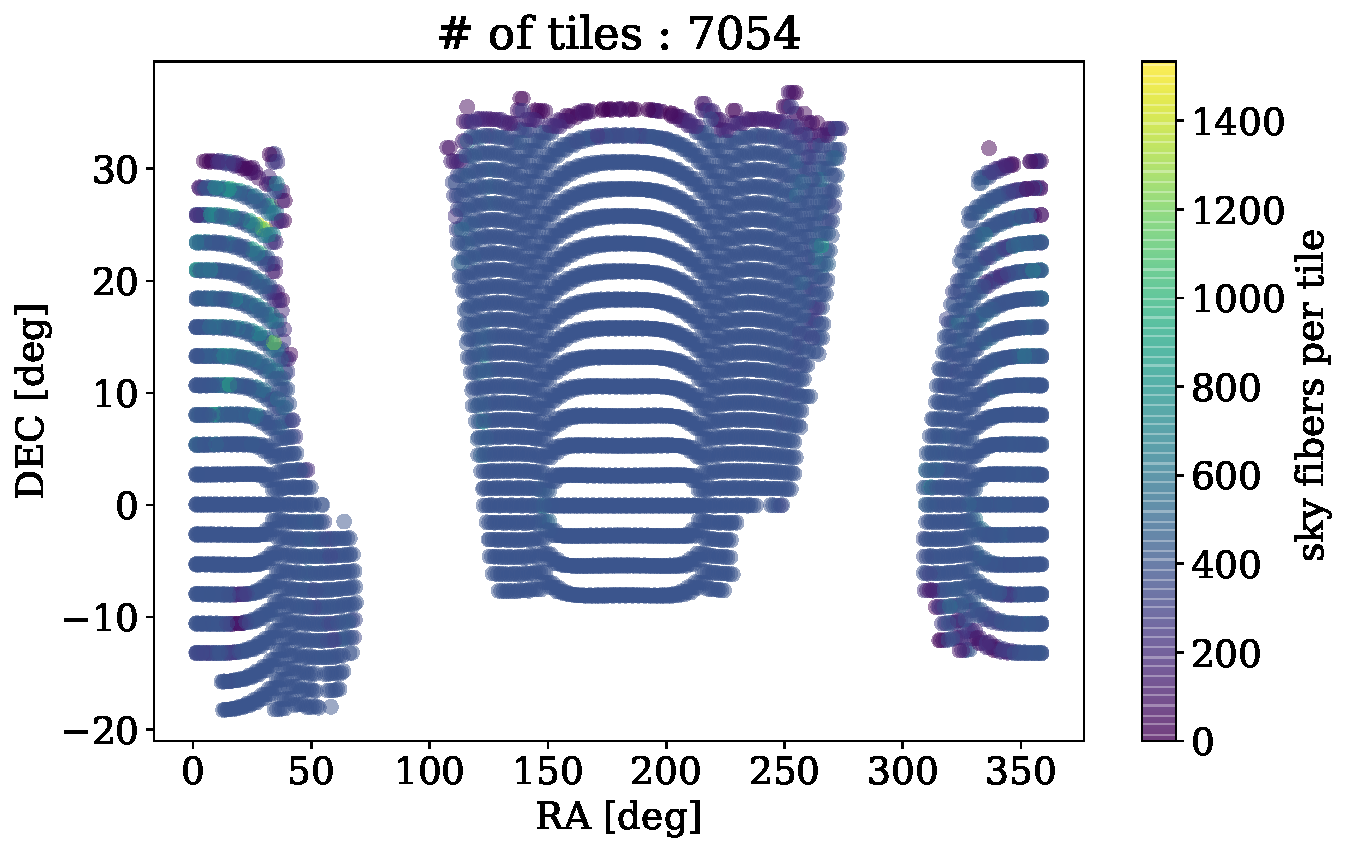
\includegraphics[scale=0.60]{assigned_sky_ra_dec_all.pdf}
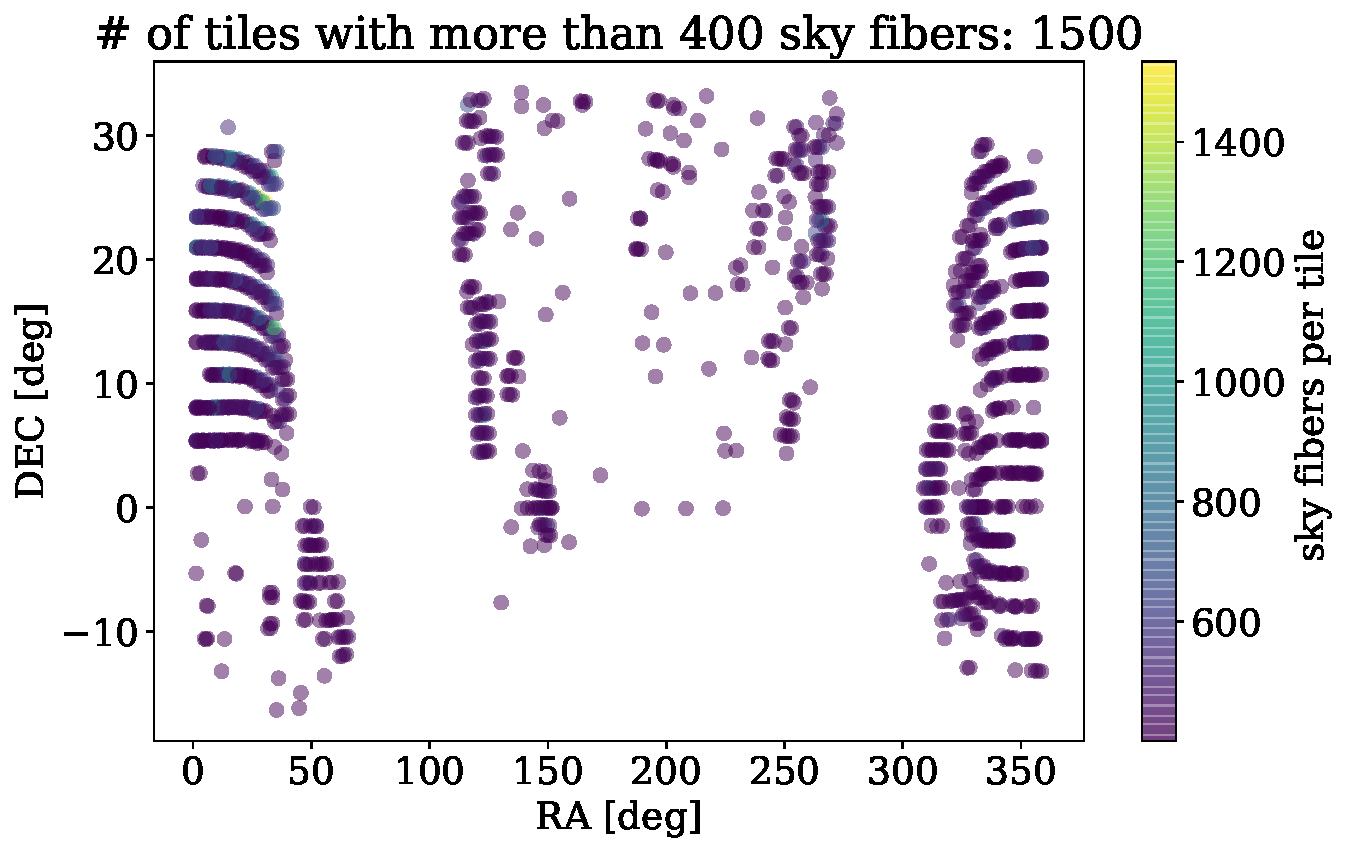
\includegraphics[scale=0.60]{assigned_sky_ra_dec_above.pdf}
\end{center}
\caption{Same as Figure \ref{fig:used_fibers}, only for SKY fibers.
The upper panel shows the sky fibers for all tiles.
The lower panel shows the tiles with at least 400 SKY fibers.
\label{fig:used_sky_fibers}}
\end{center}
\end{figure}


\begin{figure}[!h]
\begin{center}
\begin{center}
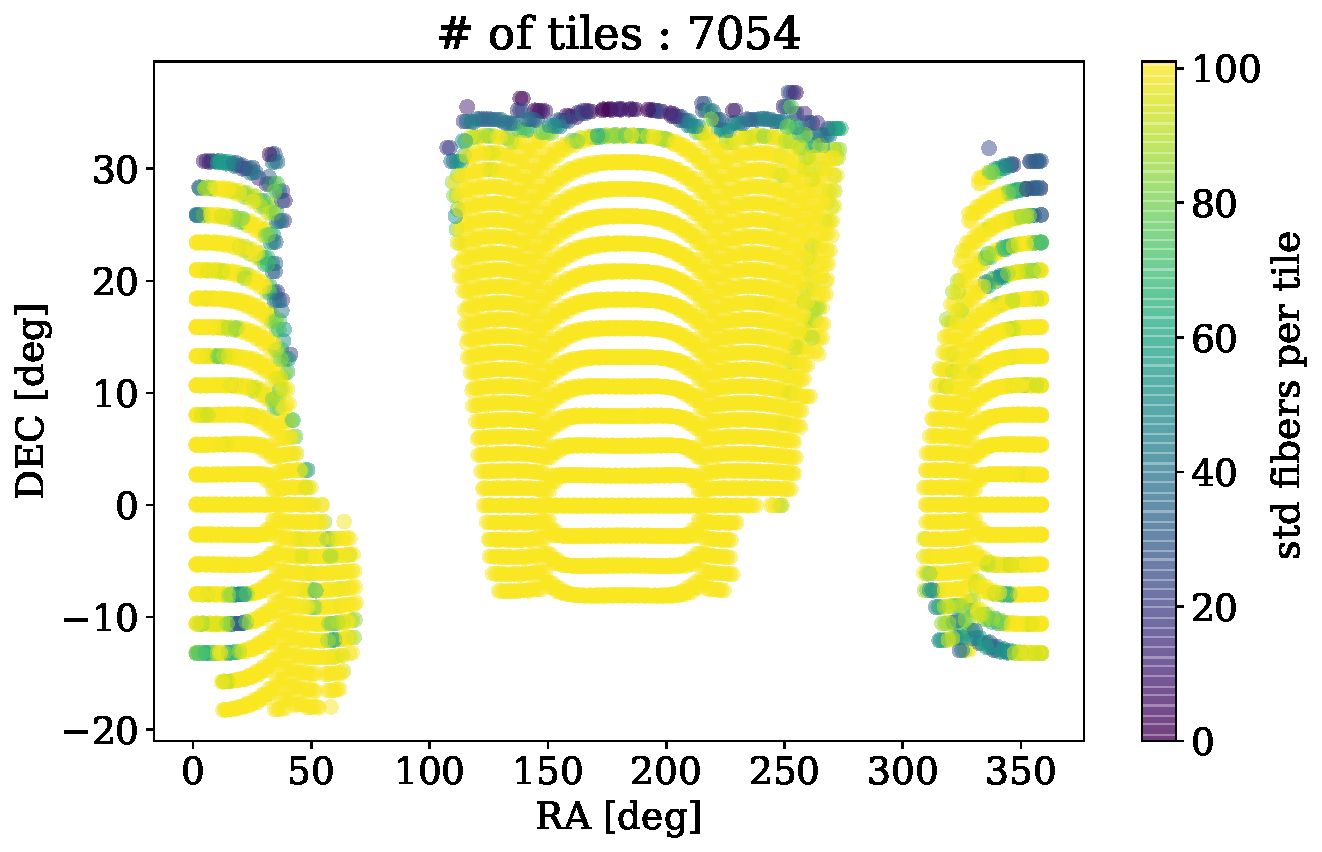
\includegraphics[scale=0.60]{assigned_std_ra_dec_all.pdf}
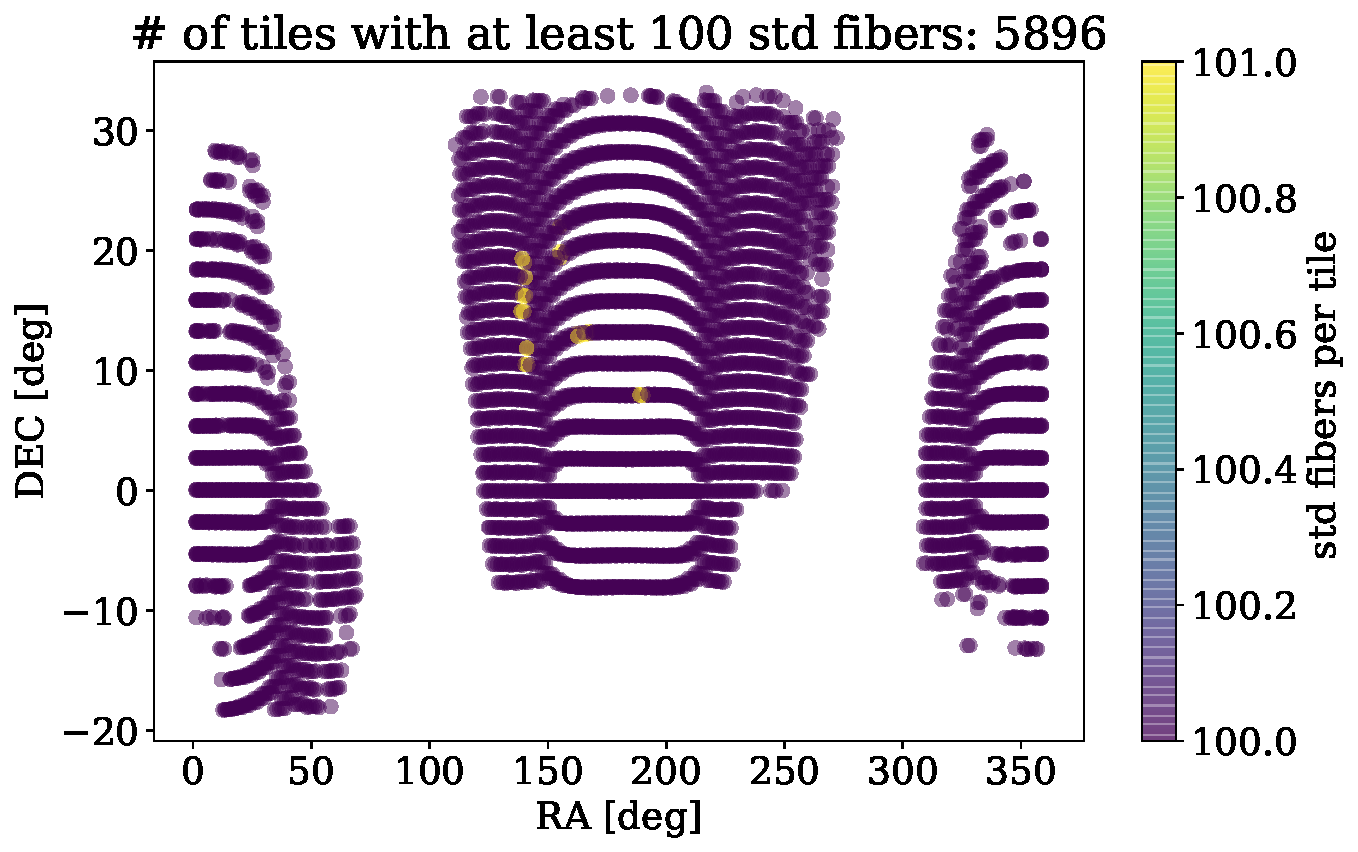
\includegraphics[scale=0.60]{assigned_std_ra_dec_above.pdf}
\end{center}
\caption{Same as Figure \ref{fig:used_sky_fibers}, only for STD fibers.
The upper panel shows the STD fibers for all tiles.
The lower panel shows the tiles with at least 100 STD fibers.
\label{fig:used_std_fibers}}
\end{center}
\end{figure}

\begin{figure}[!h]
\begin{center}
\begin{center}
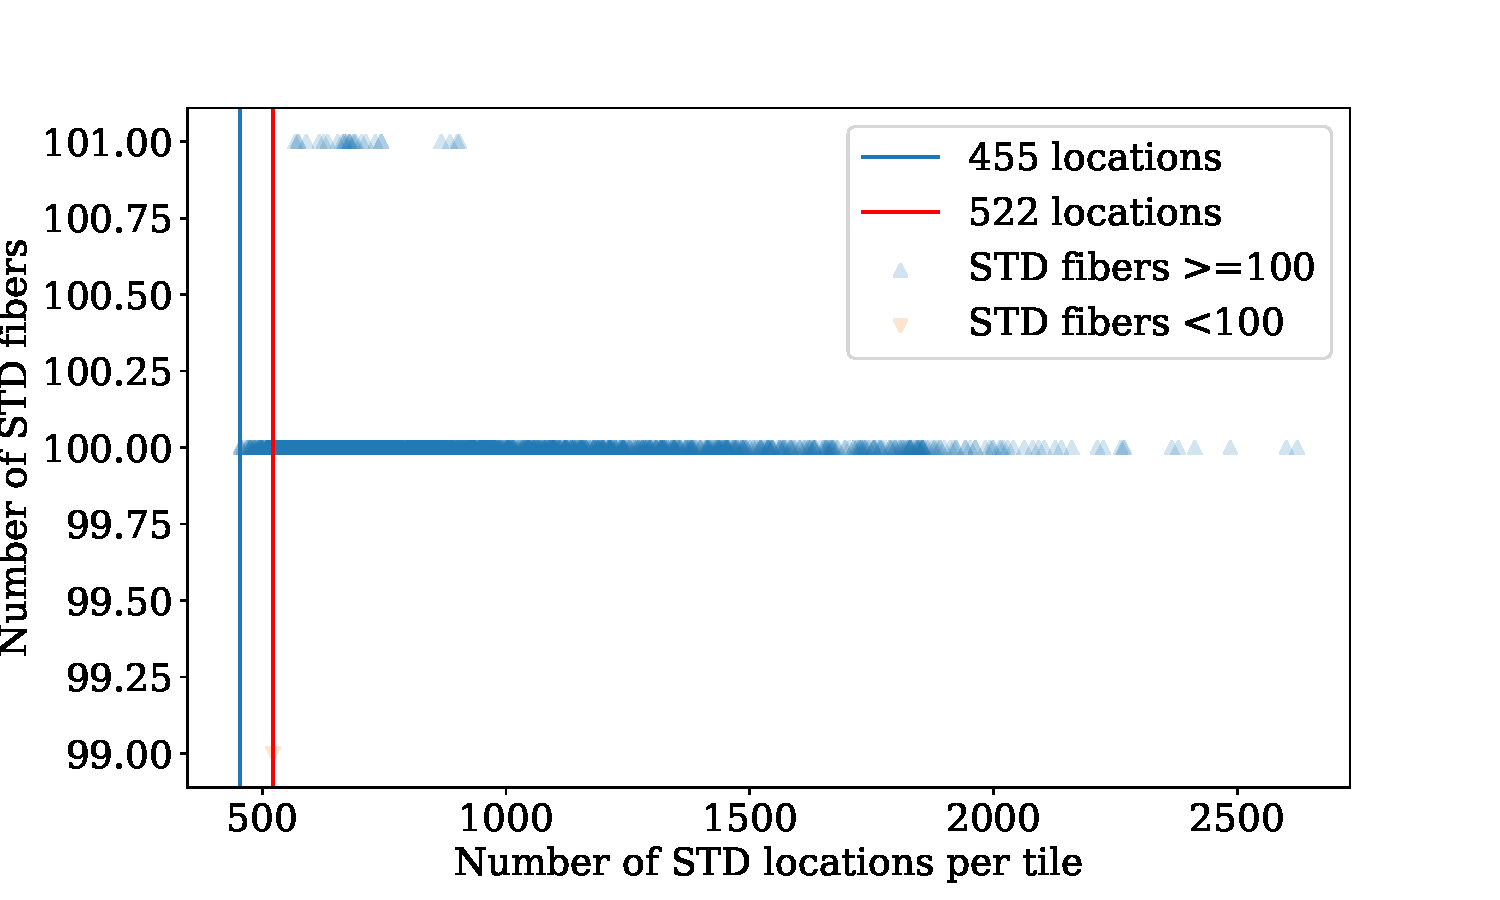
\includegraphics[scale=0.40]{std_density.pdf}
\end{center}
\caption{Number of STD fibers as a function of number of STD targets
  per tile. 
The blue line indicates the value below which the value of 100 STD
targets cannot be met. 
The red line indicates the value above which the value of 100 STD
target can always be met.
\label{fig:std_dens}}
\end{center}
\end{figure}


\begin{figure}[!h]
\begin{center}
\begin{center}
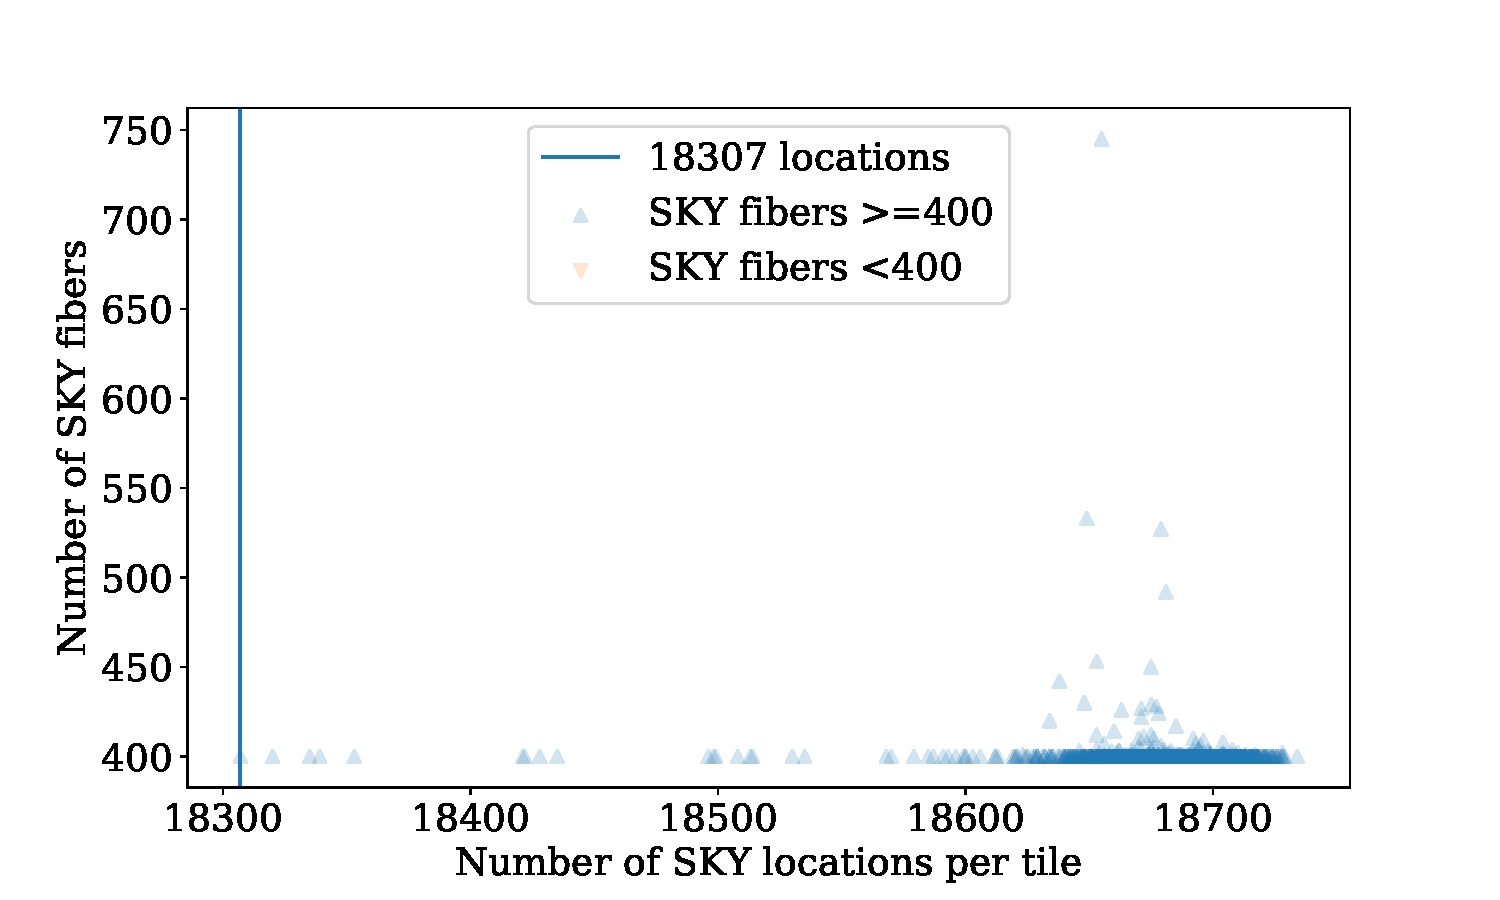
\includegraphics[scale=0.40]{sky_density.pdf}
\end{center}
\caption{Number of SKY fibers as a function of number of SKY locations
  per tile. 
The blue line indicates the value below which the value of 400 SKY 
locations cannot be met. 
The red line indicates the value above which the value of 400 SKY
locations can always be met.
\label{fig:sky_dens}}
\end{center}
\end{figure}


\end{document}



Figure \ref{fig:single_tile} show the results from an individual
tile that meets the requirements.
 
Each panel shows different kinds of targes: 
\begin{itemize}
\item SKY: fibers for sky calibration.
\item STD: fibers on standard stars.
\item BADSKY: fibers on BADSKY locations

\item SCIENCE: fibers on science targets.
\end{itemize}

\begin{figure}[!h]
\begin{center}
\begin{center}
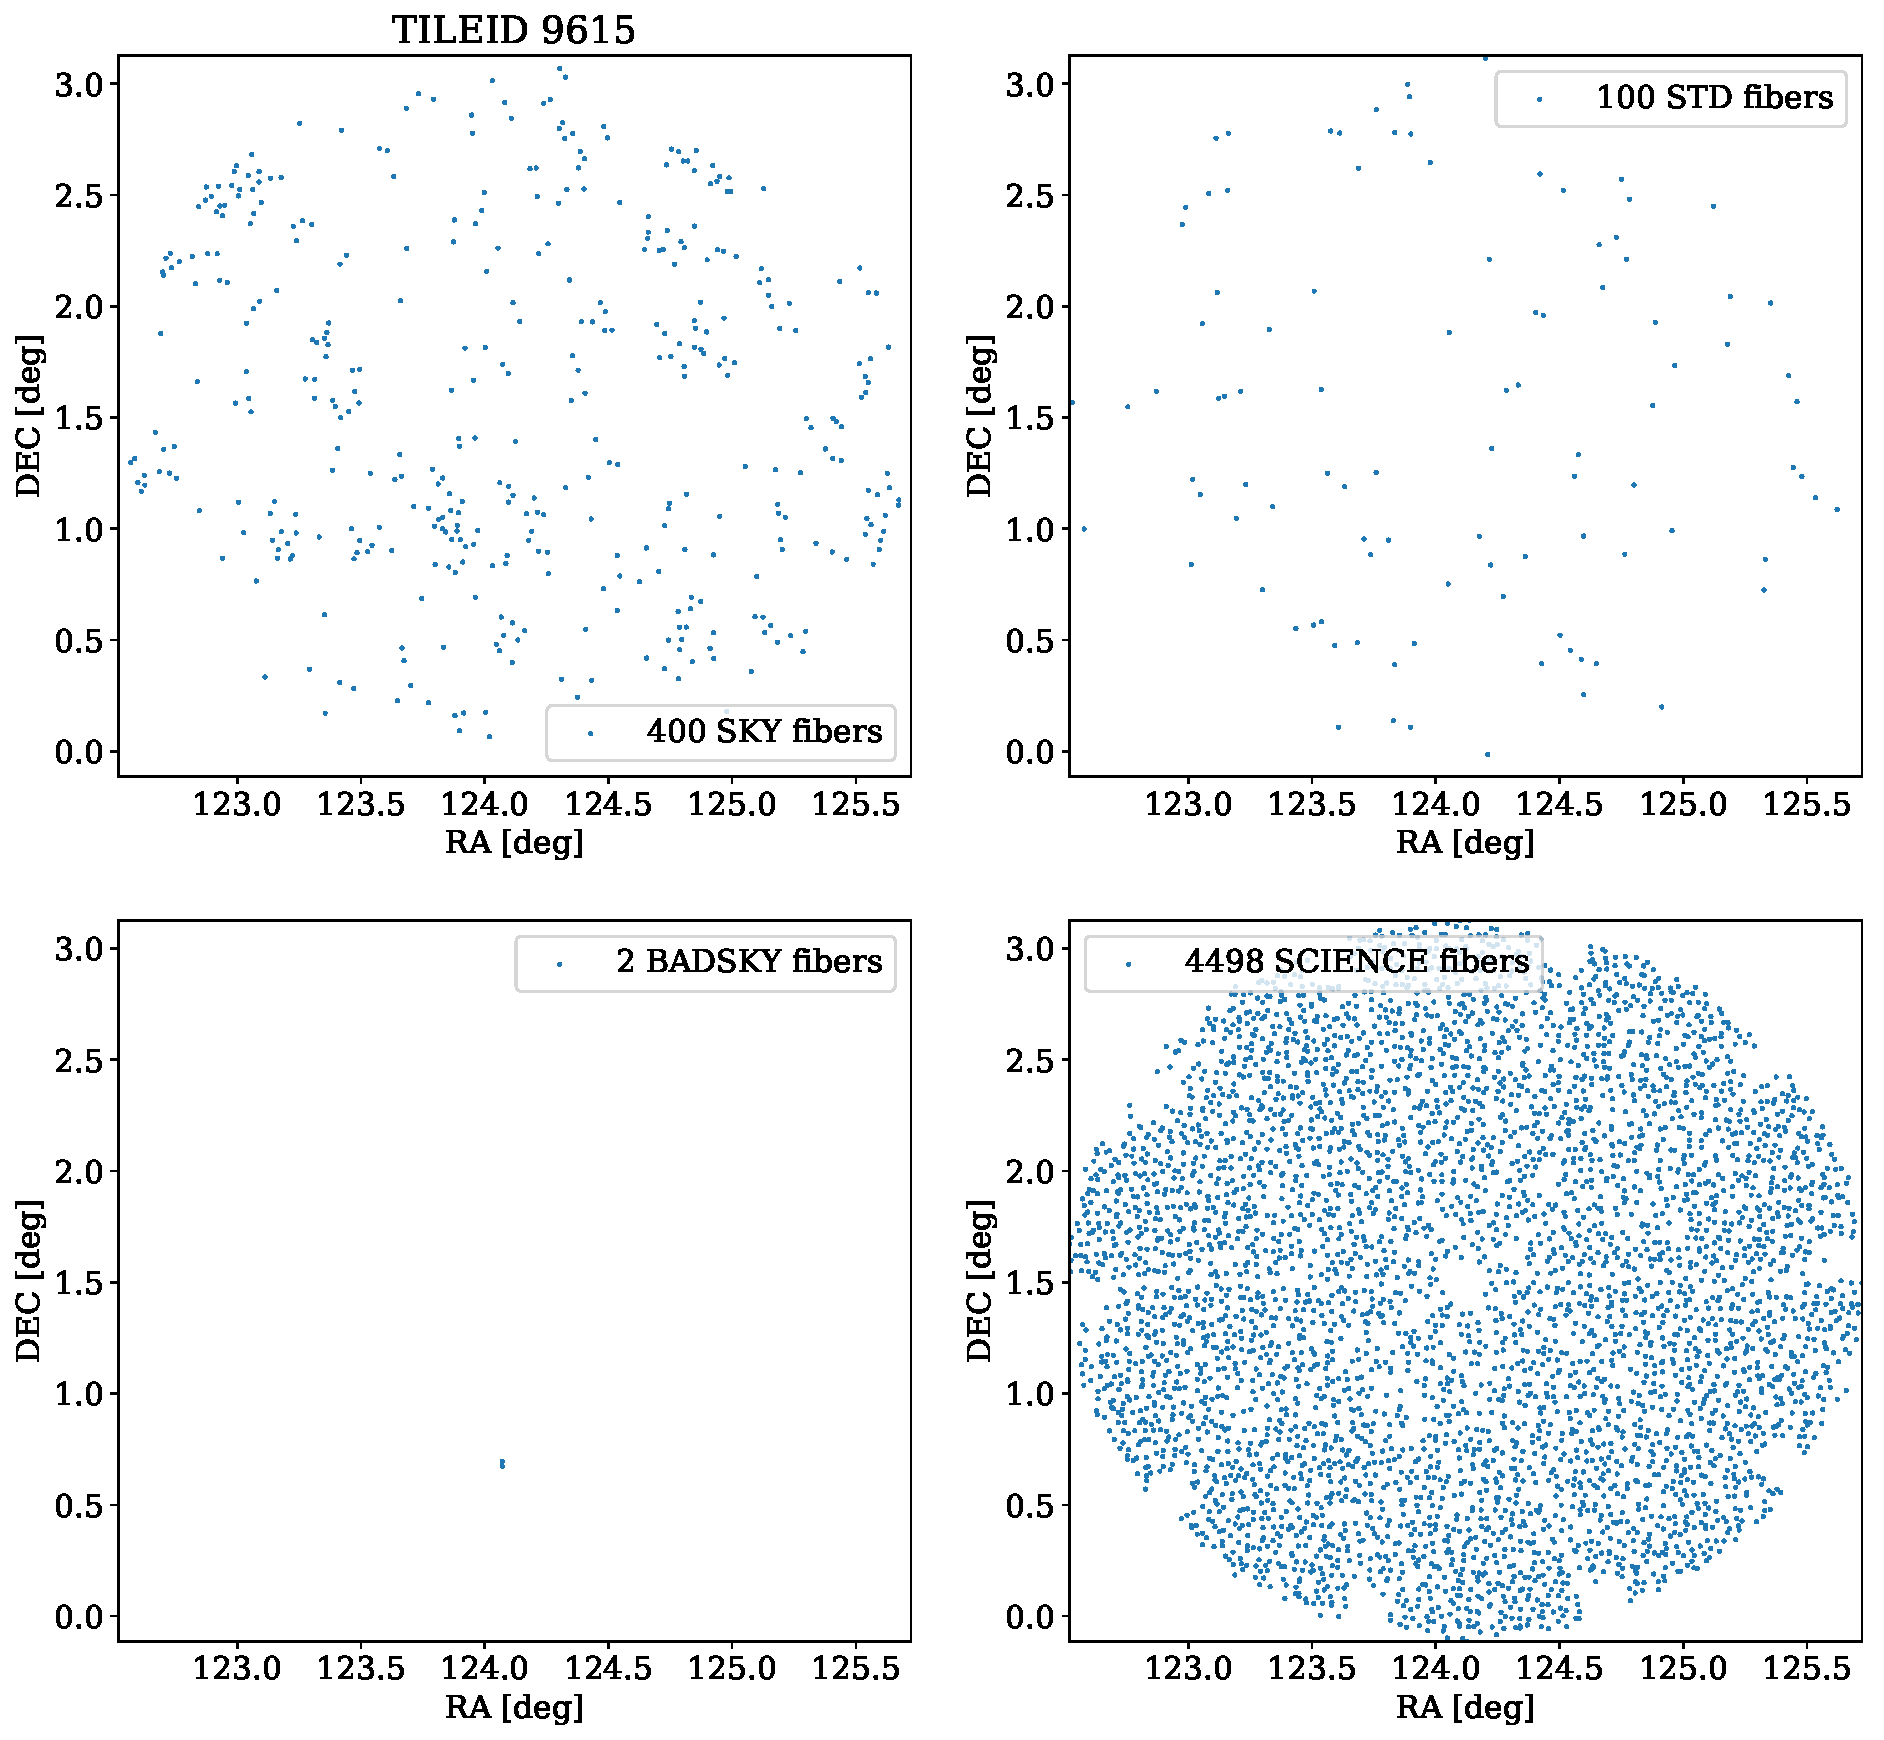
\includegraphics[scale=0.40]{single_tile_9615.pdf}
\end{center}
\caption{Tile meeting the requirements for SKY and STD fibers.
Each panel shows the different kinds of targets that are stored
in the outputs. 
\label{fig:single_tile}}
\end{center}
\end{figure}

The label shows the average and the standard deviation computed over
the tiles. 
This Figure shows that on average $99.92\%$ of the fibers are used,
on average $397$ are used for sky locations and $99$ are used for
standard stars. 
On average $4499$ science targets are observed per tile.
The small fluctuations in the number of sky location and standard star fibers
is due to changes in the input number densities for those targets. 
The input sky and stdstar catalogs must be tuned to have everywhere
the desired number of targets per tile. 

Figure \ref{fig:used_ra_dec} demonstrates that fiber assignement uses
the required fraction of fibers and provides sufficient calibration
targets. 


\section{Performance}
Runnig fiberassign on a cori login node takes 2 hours and  uses a
peak of 38GB of RAM.
The wallclock time is proportional to the number
of tiles. In this case we have that the code assigns on average one
tile per second. 
